\chapter{Determining the presence of NLOS component}

The CSI processing approaches and radar algorithms presented in the previous sections were evaluated with real measurements obtained using Nokia's ISAC FR2 proof-of-concept described in Section \ref{sec:intro-PoCarchitecture}.

\section{Measurements setup}
\label{sec:Test1_meas_scenario}

The system was mounted in an indoor industrial test facility, with gNB and sniffer positioned at a height of $5,12$ m. The transmitter was oriented towards a wide  indoor area free of obstacles. The antenna pole was located approximately 23 metres away from a warehouse rack (which was in front of a wall) and a cargo door.
Figure \ref{fig:Test1_arena_plan} shows a scheme of the test area layout.

The measurement area observed was free of any major obstructions or occlusions that could be used to create a non-line-of-sight scenario under normal conditions. 

The tests were carried out using:

\begin{enumerate}
	\item A human target.
	\item A strong reflector (large metal cabinet with flat surfaces).
\end{enumerate}

The direction (azimuth $\theta$ and elevation $\varphi$) of the transmitted beam was fixed for the whole measurement.

Before each test, a short calibration measure is performed, which includes only the static elements of the scenario. The calibration data will be used in the post-processing steps for clutter removal as described in Section \ref{sec:clutter_removal}.

\begin{figure}[H]
	\centering
	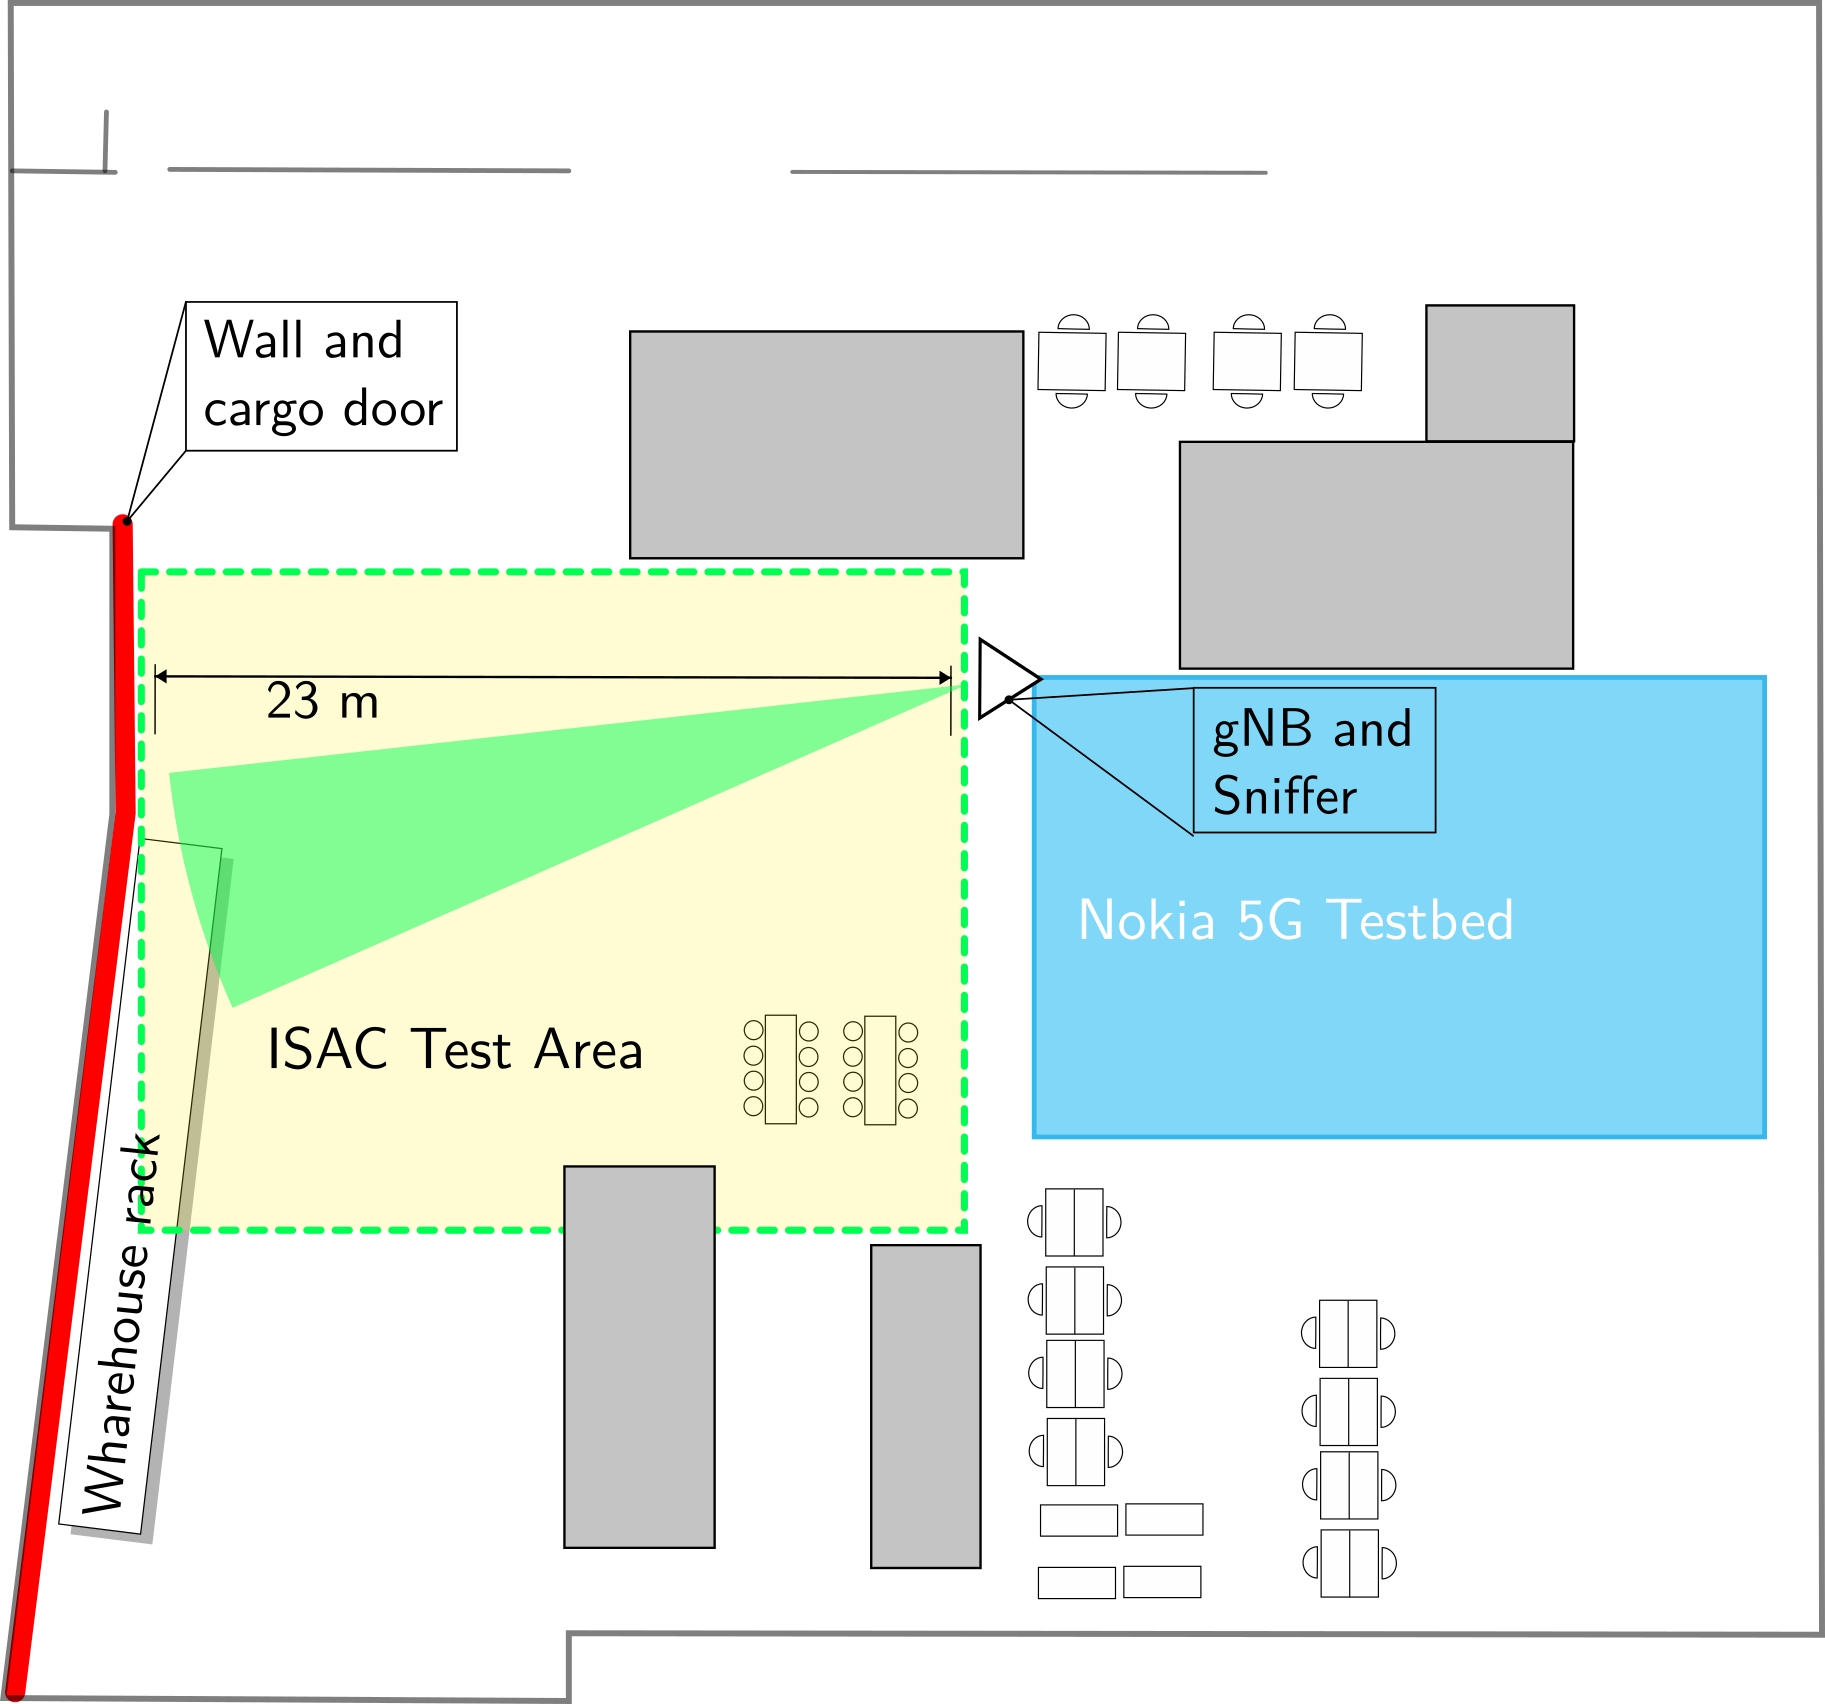
\includegraphics[width=.6\textwidth]{Images/Test1/arena_plan}
	\caption{Scheme of the PoC deployment layout in ARENA 2036, Stuttgart.}
	\label{fig:Test1_arena_plan}
\end{figure}


\begin{figure}[H]
	\centering
	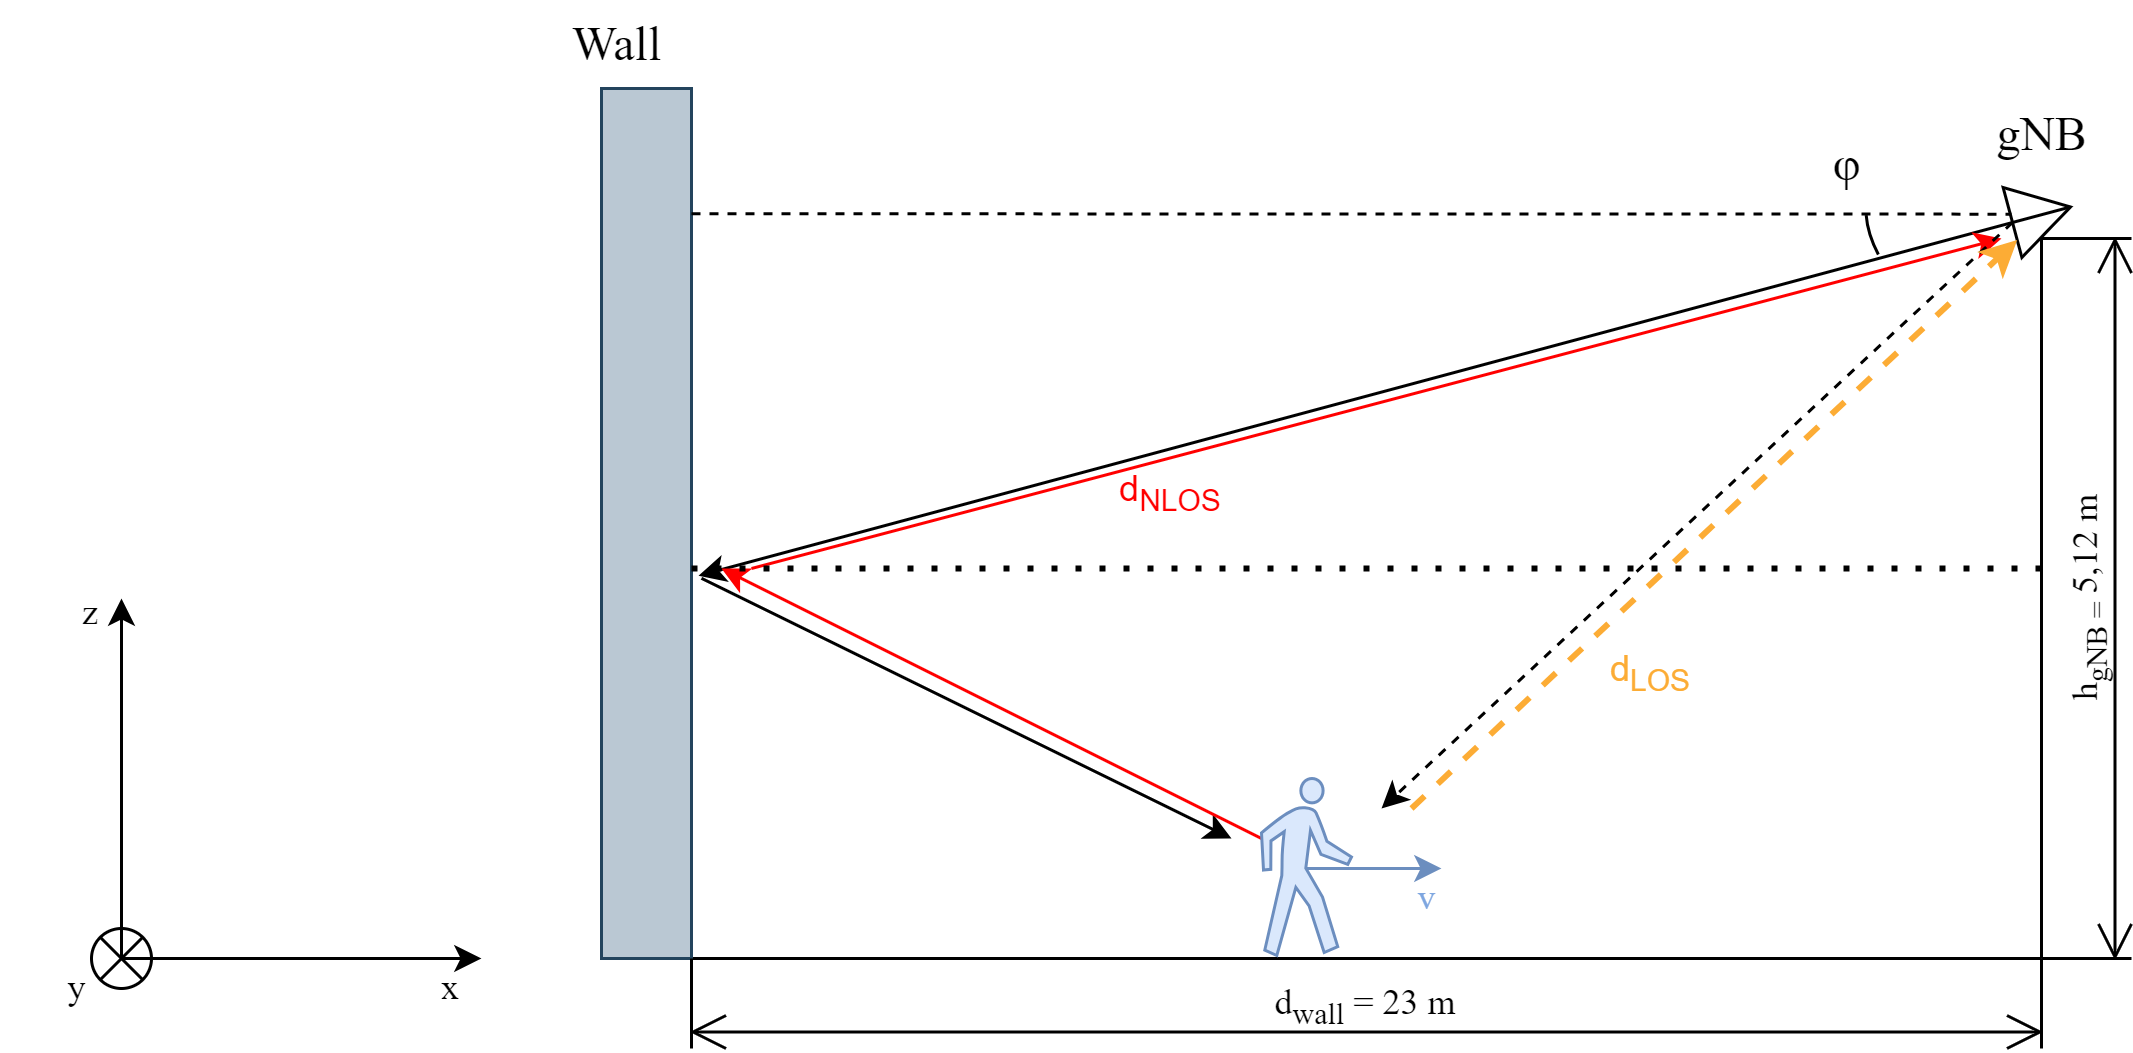
\includegraphics[width=1\textwidth]{Images/Test1/base-lateral_view_los_geometry}
	\caption{Lateral view of measurement scenario. NLOS return (red) is coupled with a LOS component (orange) generated from the secondary lobe.}
	\label{fig:Test1_base-lateral_view}
\end{figure}

\section{Measurement Scope: Detection Rate}

The radar system using OFDM can determine the range and radial speed of a target. In this case with a fixed angle of arrival (AOA). If an object moves azimuthally within the transmitted beam, it will appear static to the sensing system.

The test aimed to maximize the radial speed of the target to analyse the characteristics of the signal generated by its reflection.

During the initial measurement, the antenna boresight was directed perpendicular to the wall, while the target moved radially between the transmitter and reflector. The test subject moved towards the gNB and back multiple times in a straight line during the measurements.

\begin{figure}[H]
	\centering
	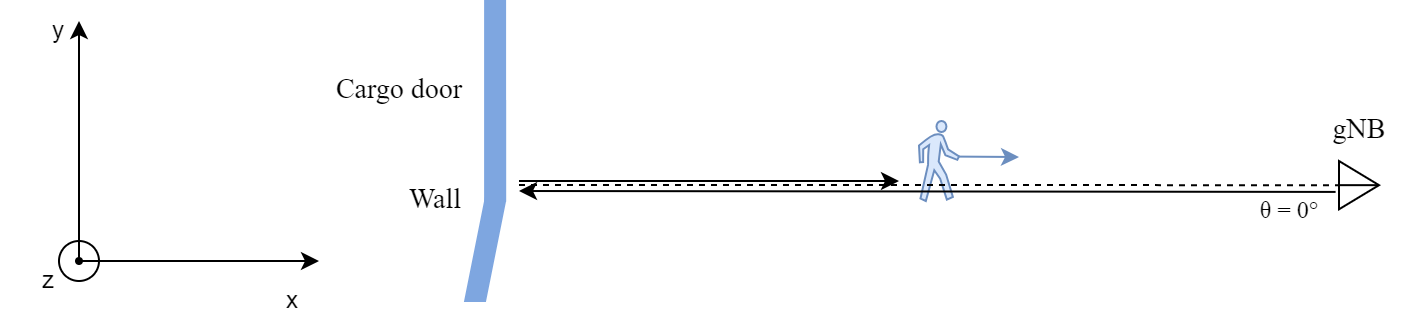
\includegraphics[width=1\textwidth]{Images/Test1/base-top_view}
	\caption{Top view of measurement scenario.}
	\label{fig:Test1_base-top_view}
\end{figure}


The beam elevation was chosen to be as high as possible to pass over the target and reflect on the wall, simulating a non-line-of-sight (NLOS) environment.

Due to the rather large beamwidth of the system, $\pm$7\textdegree\hspace{1pt} in azimuth and elevation, and its sidelobes, the measurement observed the presence of a LOS target return in addition to the expected NLOS one generated by reflection.

During the measurement, the direct component was always visible as no other obstacle was positioned in the scene. It was then decided to use this component and the knowledge of the geometry of the test area to obtain an estimate of the position and velocity of the NLOS return. This estimate was used to check if any of the detected peaks corresponded to the moving target.
The direct target return provided additional information, which was then used as ground truth to determine the correct position of the person within the test area.
Figures \ref{fig:Test1_base-lateral_view} and \ref{fig:Test1_base-top_view} depict a scheme of the measurement.

\begin{itemize}
	\item Speed of the NLOS component was estimated as:
	$$ \hat{v}_{\text{NLOS}} = -v_{\text{LOS}}$$
	since the direct and reflected beams will hit the target from the opposite direction.
	\item Range of the NLOS component was estimated considering the model in Figure \ref{fig:Test1_base-lateral_view} as:
	$$ \hat{d}_{\text{NLOS}} = 2 d_{\text{wall}} - d_{\text{LOS}}\cdot \cos{(\arctan{\left(\frac{h_{\text{gNB}}}{d_{LOS}}\right)})}$$
\end{itemize}


\textit{Detection rate} was defined as the metric used to evaluate the experiment: if the speed and range of the NLOS return matched the expected values calculated from the LOS data, detection was considered positive.
The detection rate was then obtained as the ratio between the number of frames in which the NLOS component was above threshold, and the total number of frames in which the LOS component was detected.


\begin{equation*}
	\text{Detection rate} = \frac{\text{frames with NLOS}}{\text{frames with LOS}}
\end{equation*}

Due to the multiple reflections, the NLOS return presented considerably smaller power compared to LOS.
This meant that due to the presence of large clutter returns and their sidelobes, this return is not necessarily the strongest one in the NLOS region of the periodogram.
Detection rate was hence evaluated comparing the five strongest returns in NLOS with the estimated position of the target.

\subsection{Processing of the NLOS region}

After defining the two regions of interest from the periodogram and discarding the static components, as described in Section \ref{sec:los_nlos_separation}, peak detection is conducted separately for each region. 

%The chosen detection strategy was CA-CFAR, which utilized a square contribution window and a probability of false alarm $p_{\text{FA}} = 10^{-6}$. The size of the CA-CFAR window was set depending on the width of the target in speed bins, which depended on number of processed frames and OFDM sampled symbols.

\begin{figure}[H]
	\centering
	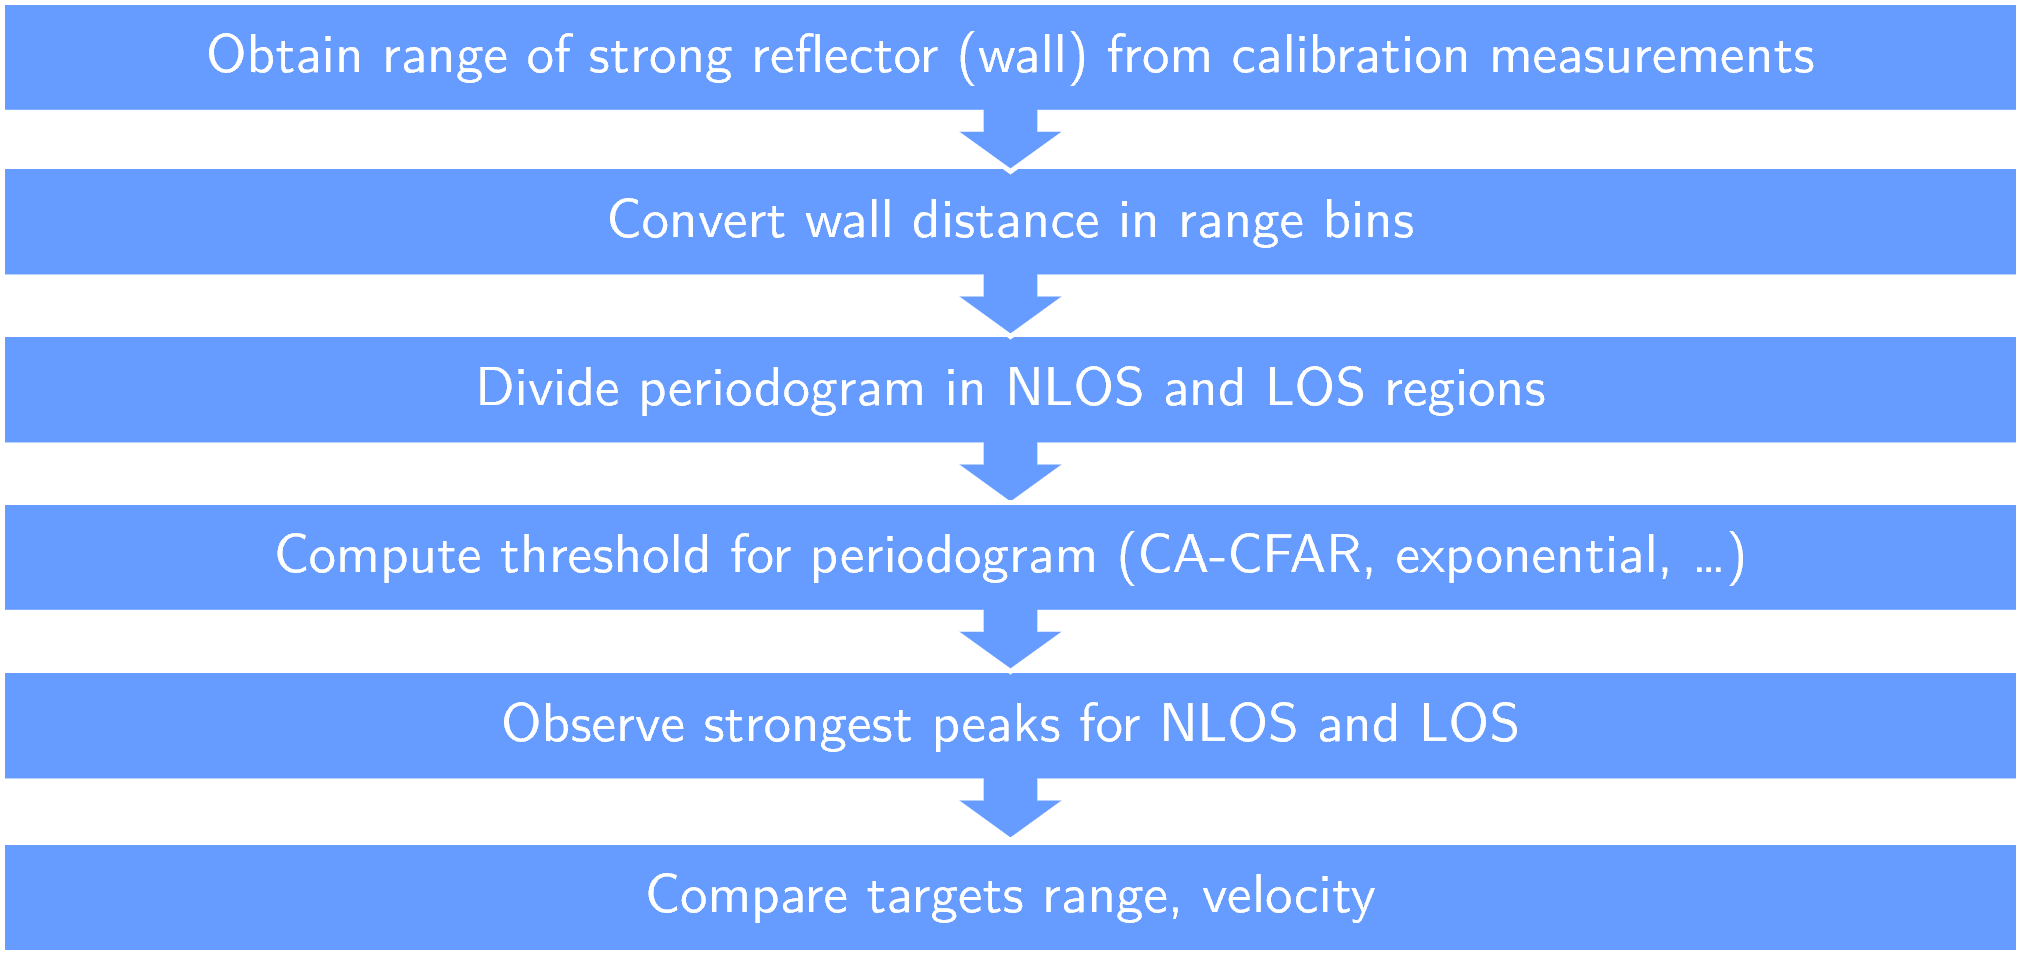
\includegraphics[width=0.8\textwidth]{Images/Test1/NLOS-proc-pipeline_wide_text12.png}
	\caption{Periodogram processing pipeline used for detection tests.}
	\label{fig:Test1_NLOS-proc-pipeline}
\end{figure}

A standard strongest peak search is performed for the LOS region, while multiple peak detection is conducted in NLOS. Only the five strongest peaks were considered, this assumption was made since the test was conducted in a single target scenario.
Accurate range and velocity measurements are obtained after interpolation of each peak with the adjacent bins.

The full process for the experiment is summarized in figure \ref{fig:Test1_NLOS-proc-pipeline}.

% TODO: add info on target dimensions for CA-CFAR, human case since guard cells were set in meters


\section{Observation on detection rate of a strong reflector}

The first measurement was conducted using the strong reflector, which represented an ideal scenario.


\begin{figure}[H]
	\centering
	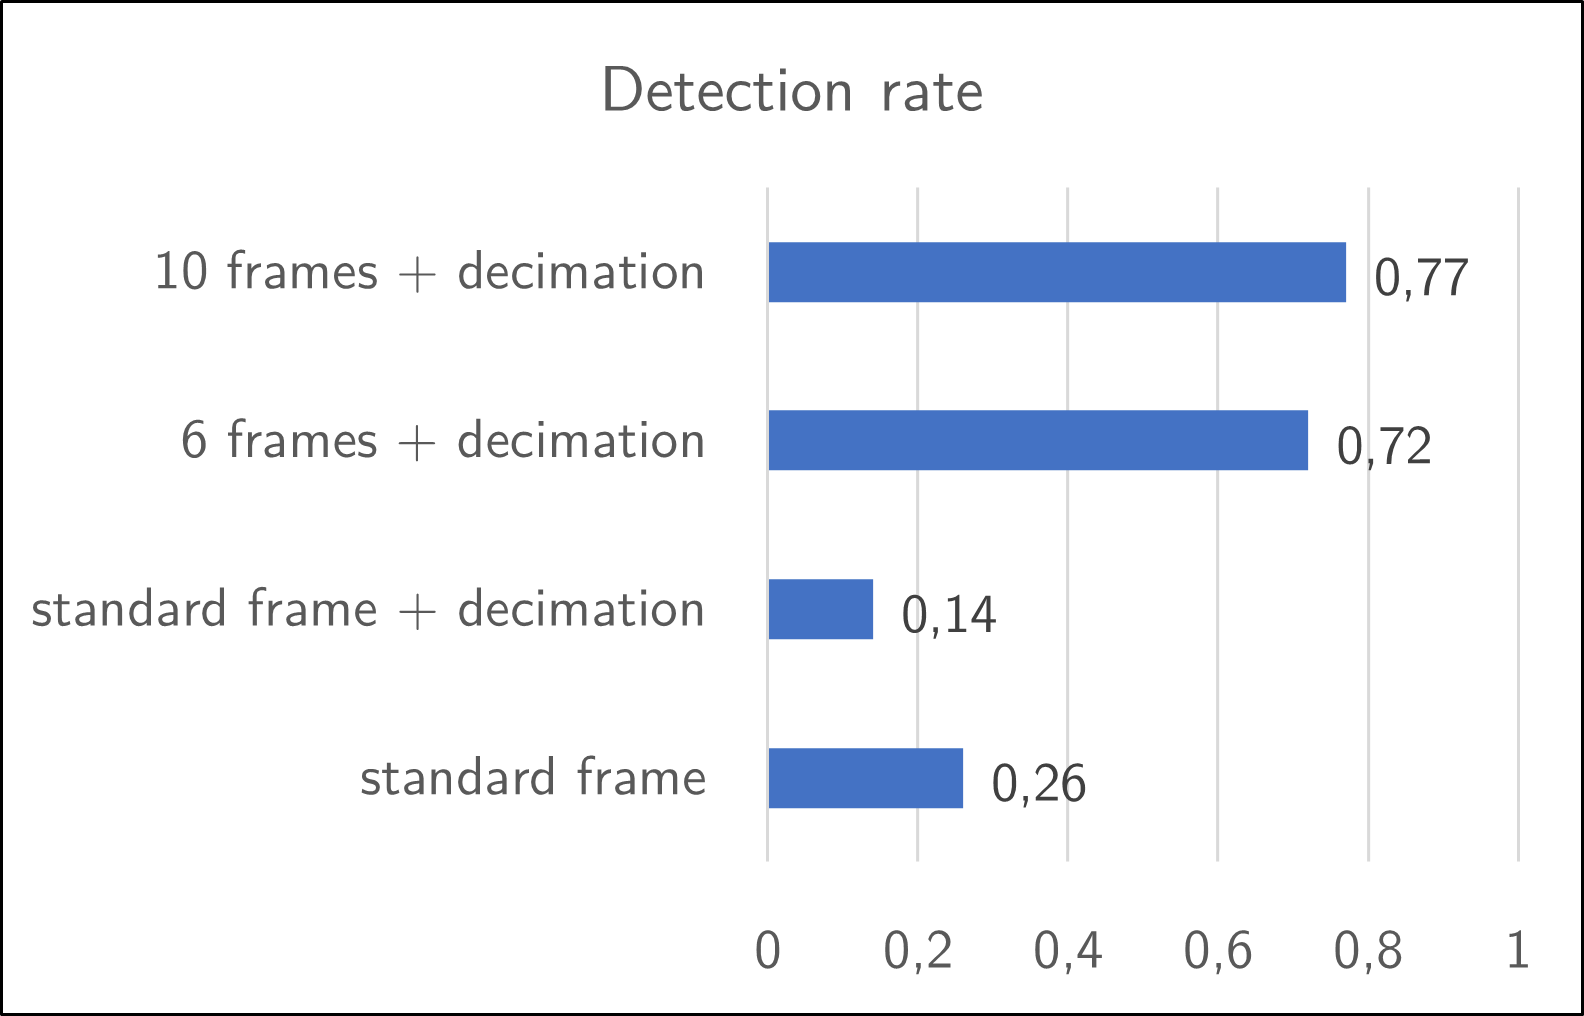
\includegraphics[width=0.7\textwidth]{Images/Test1/detect_hist_strong_ref.png}
	\caption{Detection rate observed for passive metal reflector target in mixed LOS/NLOS measurement.}
	\label{fig:Test1_detect_rate_strong_ref}
\end{figure}

The detection rate test displayed in figure \ref{fig:Test1_detect_rate_strong_ref} shows that the passive reflector, thanks to its significantly larger radar cross section, is clearly identified while it is moving and is not masked by clutter.

Passing the NLOS measurements to a Kalman filter it was possible to track the target in the range/Doppler plane, as shown in figure \ref{fig:Test1_kf_track_strong_ref}. This result is to show that one of the main limitation of NLOS signals is the strength of the target return. Objects with large RCS are easier to separate from the noisy background and the effect of fading and obstruction is relatively small.

\begin{figure}[H]
	\centering
	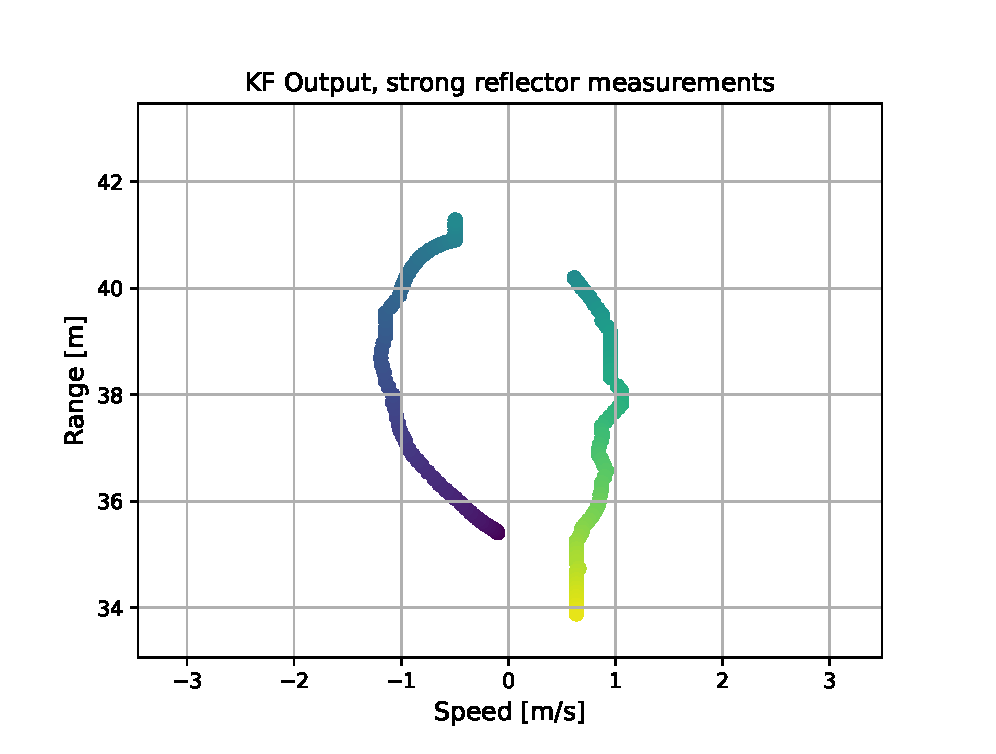
\includegraphics[width=0.7\textwidth]{Images/Test1/kf_track.eps}
	\caption{Output of KF tracking the target in the range/speed plane.}
	\label{fig:Test1_kf_track_strong_ref}
\end{figure}


\subsection{Scope of the measurement - Detection rate}

The results were obtained with the different frame processing strategies presented in chapter \ref{chap:TDD pattern of the OFDM frame}. When combining subsequent frames to increase time-aperture, the window processing stride was set to be lower then the number of frames. This allowed to increase the amount of target updates.

Target detection was carried out considering the \textit{n}-strongest peaks and comparing them against the LOS data. If any of the observed NLOS peaks was deemed to be corresponding to the target then detection was positive.

\begin{figure}[H]
	\centering
	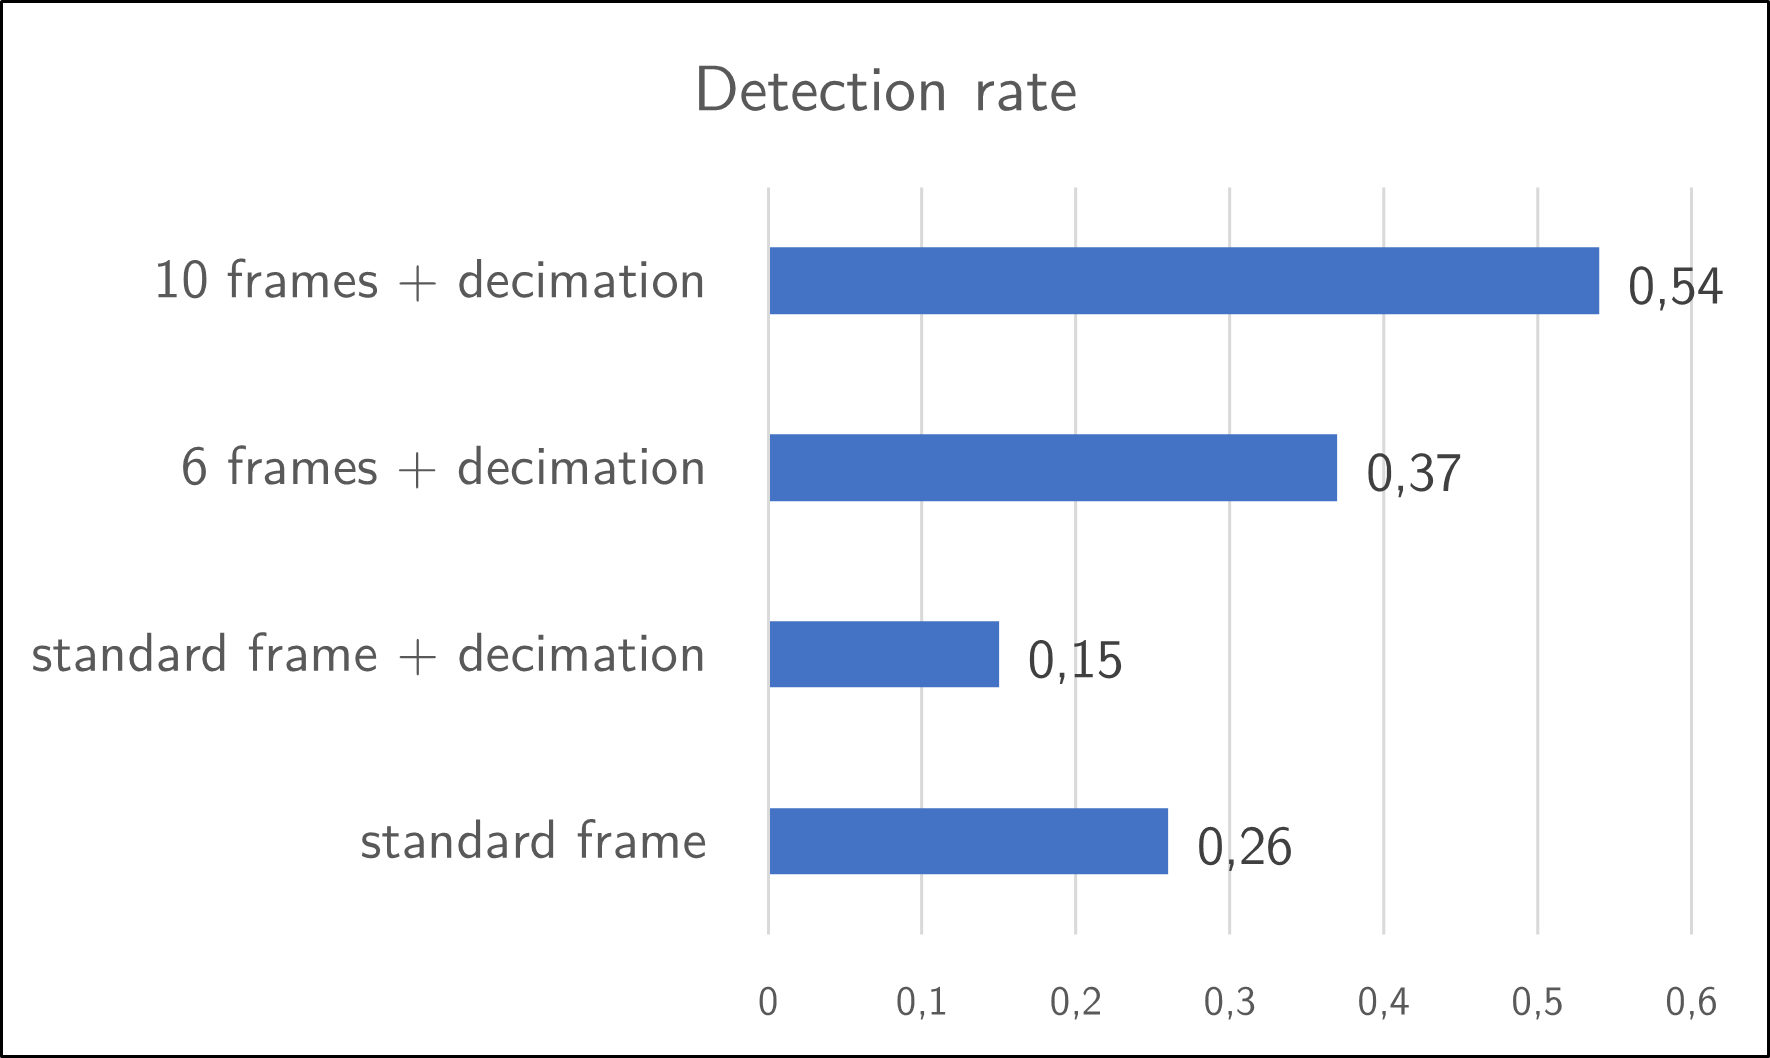
\includegraphics[width=0.7\textwidth]{Images/Test1/detect_hist.png}
	\caption{Detection rate observed for human target in mixed LOS/NLOS measurement.}
	\label{fig:Test1_detect_hist}
\end{figure}

Using a larger time-aperture significantly increased the detection rate due to the improved speed resolution. However, this approach may cause range spreading issues, particularly for fast targets. This phenomenon is not a significant drawback in NLOS sensing since the system's primary objective is target detection rather than precise tracking and positioning.

It was observed that the NLOS target return was not the strongest return in the majority of cases, with lower peak power with respect to noise and spectral artefacts, also due to channel fading.

The detection rate was observed over the whole measurement: frames in which the target changed direction and was therefore static, or presented a low speed component, were included. Processing these time instants meant that the NLOS component was likely to be masked by clutter and give a negative detection. The effective detection rate, measured only when the target is moving, is likely to be higher.

%TODO: change subsection title
\subsubsection{Moving average of detection rate}


% TODO: I don't like this phrasing
The average detection rate over 10 consecutive updates is shown in figure \ref{fig:Test1_moving_avg}. It can be seen that when the target is moving, and therefore  well separated from the clutter region, detection rate appears to be above 80\% for a number of consecutive 10-update intervals.

Although obtained in a controlled single target scenario, this measure opens the door to the possibility of determining the presence of NLOS moving targets without the aid of ground truth data.


% TODO: change picture with higher resolution one, maybe solved
\begin{figure}[H]
	\centering
	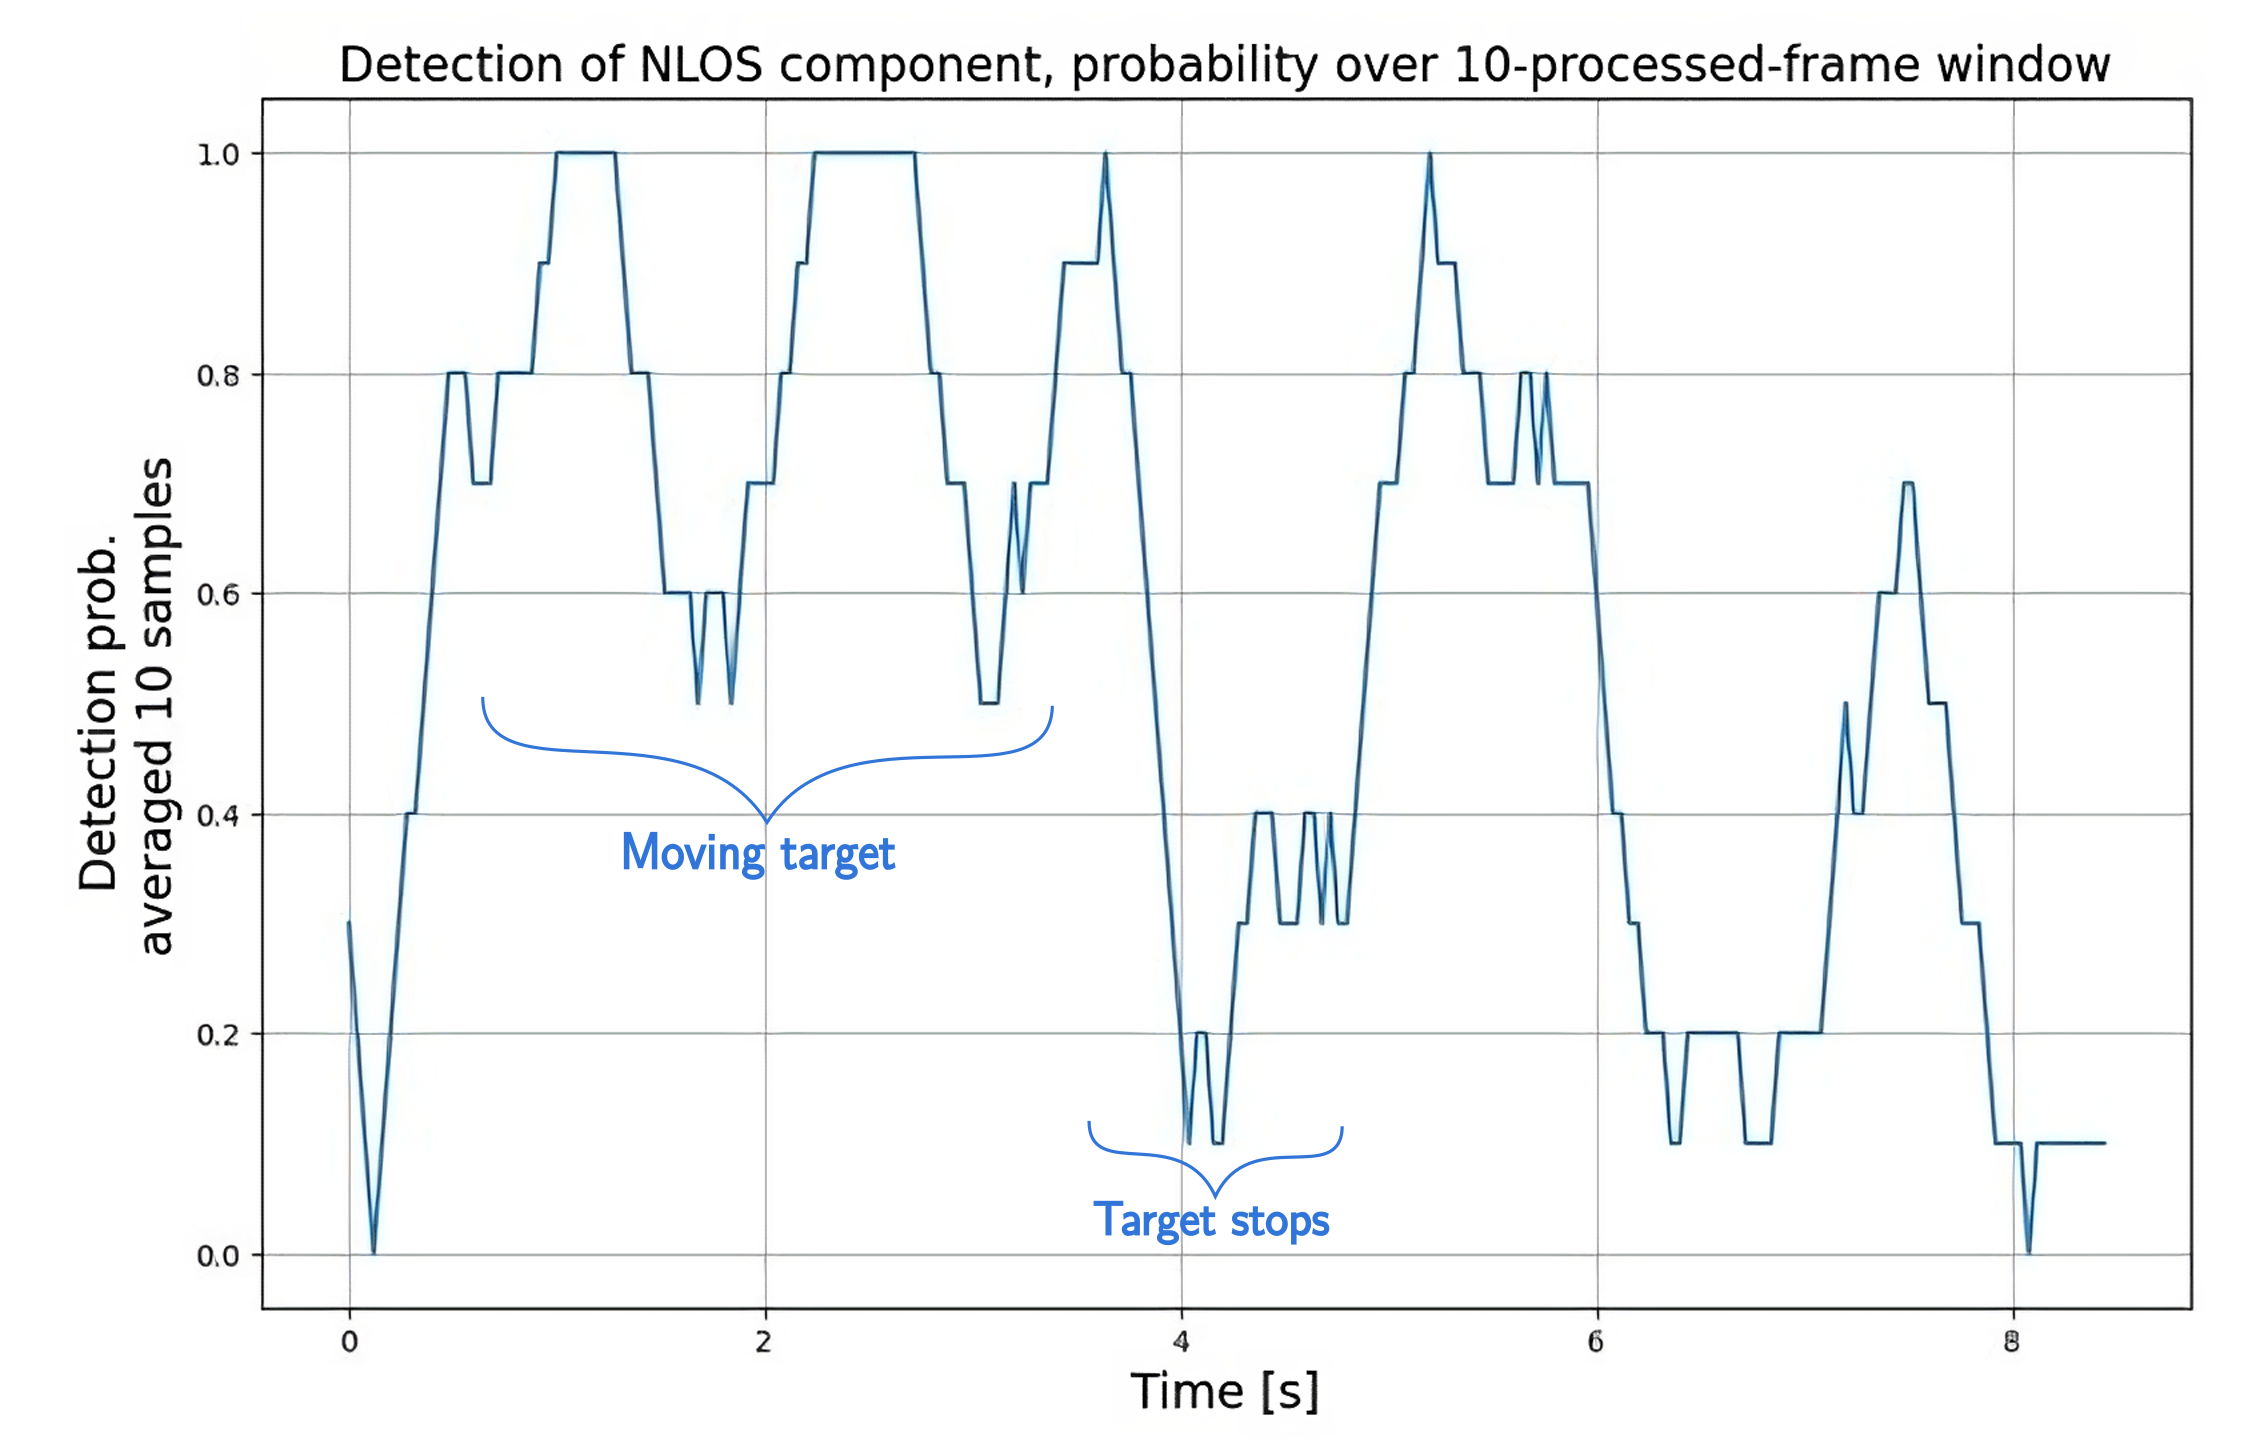
\includegraphics[width=0.7\textwidth]{Images/Test1/moving_avg-transformed_wtext}
	\caption{Detection rate observed for human target in mixed LOS/NLOS measurement.}
	\label{fig:Test1_moving_avg}
\end{figure}


